%% Chapter 6: Results
\chapter{Results}
\label{chapter:results}

\graphicspath{ {report/C6 Results/assets/} } 

** remember to include results of all early, prelim experiments including the OpenBCI experiments and periodogram plots of the alpha energy experiments with the initial Frankenstein hardware.

\section{Hardware Verification and Testing}
\subsection{Digital signal processing system}

\begin{figure}[h]
    \centering
    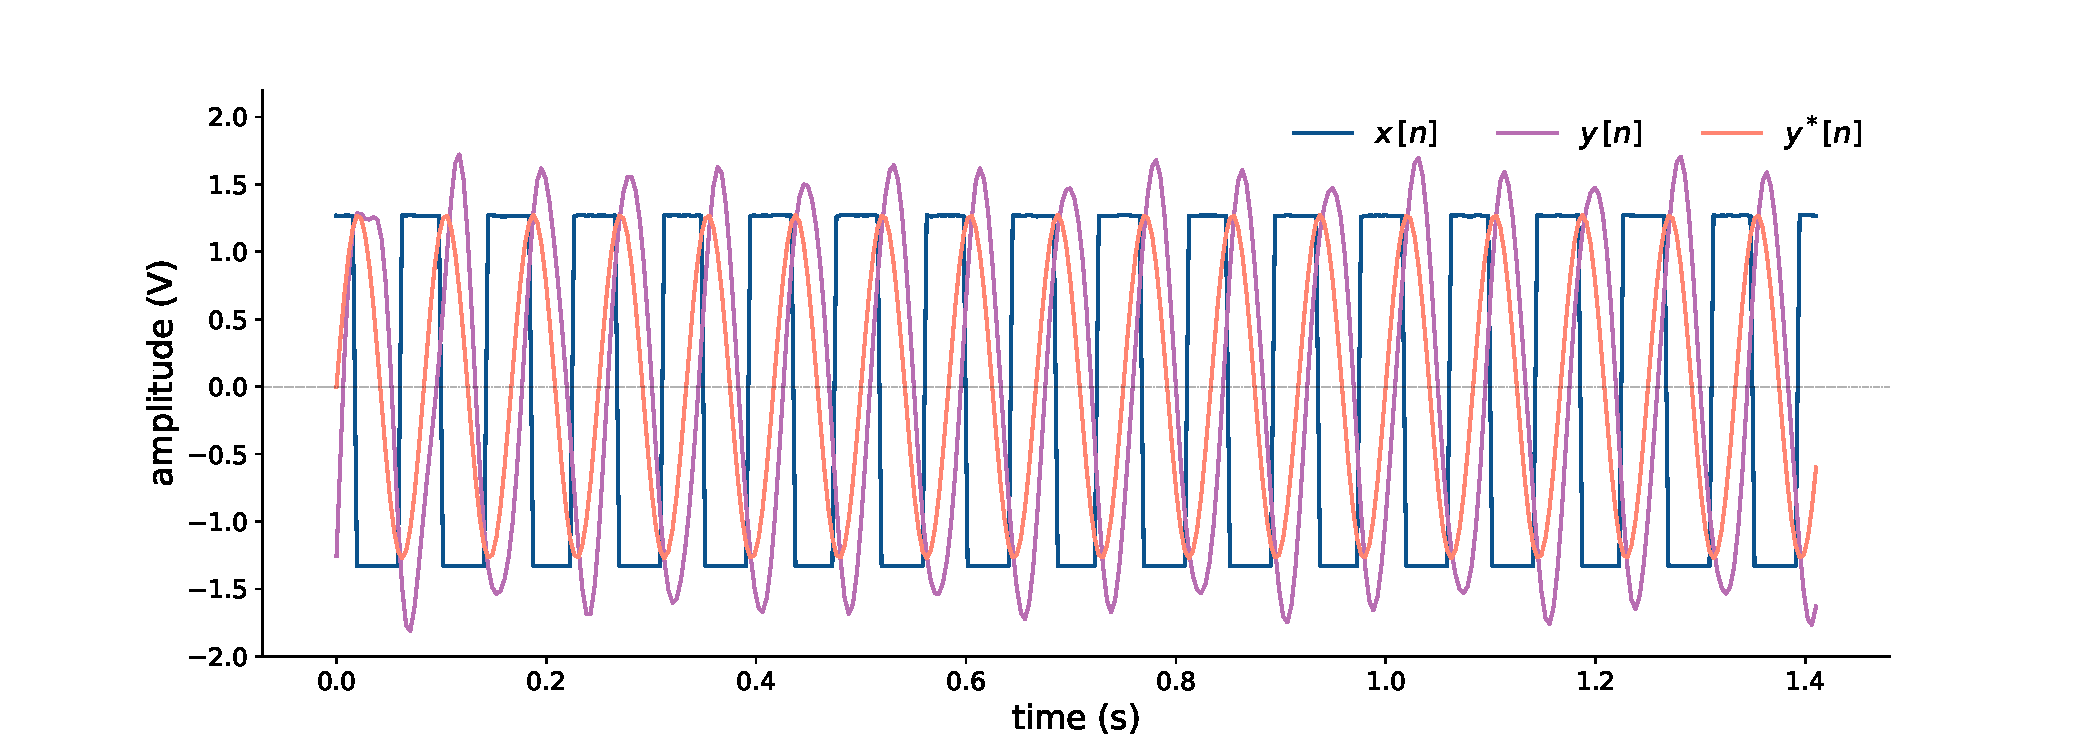
\includegraphics[width=\textwidth]{sq_wave_filtering_time}
    \caption[Time domain plot showing the measured square wave signal together with the digitally-filtered output signal.]{Time domain plot showing the measured square wave signal $x[n]$ together with the digitally-filtered output signal $y[n]$ designed to retain only the fundamental frequency $f_x^{(0)}$ of $x[n]$. The ideal output signal $y^*[n]$ represents a sinsuoid at frequency $f_x^{(0)}$: $y^*[n] = \frac{4}{\pi}sin(2\pi f_x^{(0)}n)$.}
    \label{fig:sq-wave-time-c6}
\end{figure}

\begin{figure}[h]
    \centering
    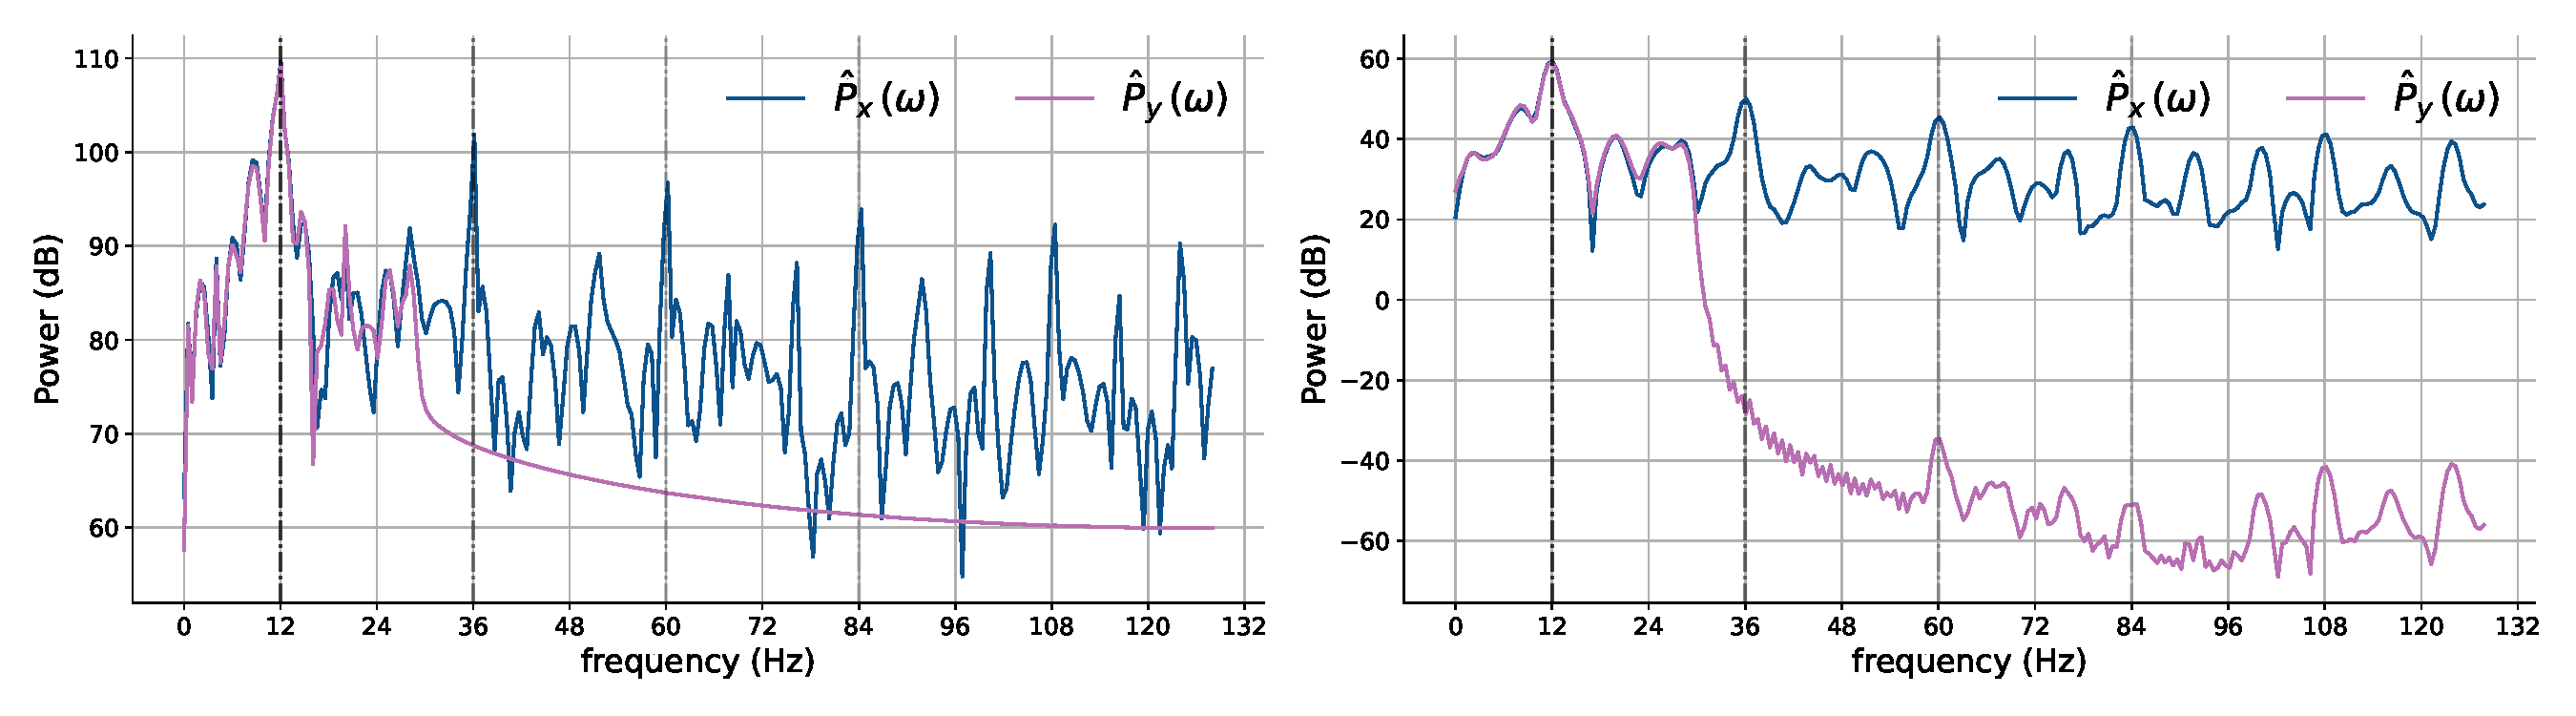
\includegraphics[width=\textwidth]{sq_wave_filtering_spectra}
    \caption[PSD estimates of a measured input signal and its filtered output]{Standard periodogram (left) and Welch-averaged periodogram (right) representing PSD estimates of measured input signal $x[n]$ and filtered output $y[n]$. Dashed vertical lines mark $f_x^{(0)}$ and odd-numbered harmonics of $x[n]$.}
    \label{fig:sq-wave-spectra-c6}
\end{figure}

\begin{figure}[h]
    \centering
    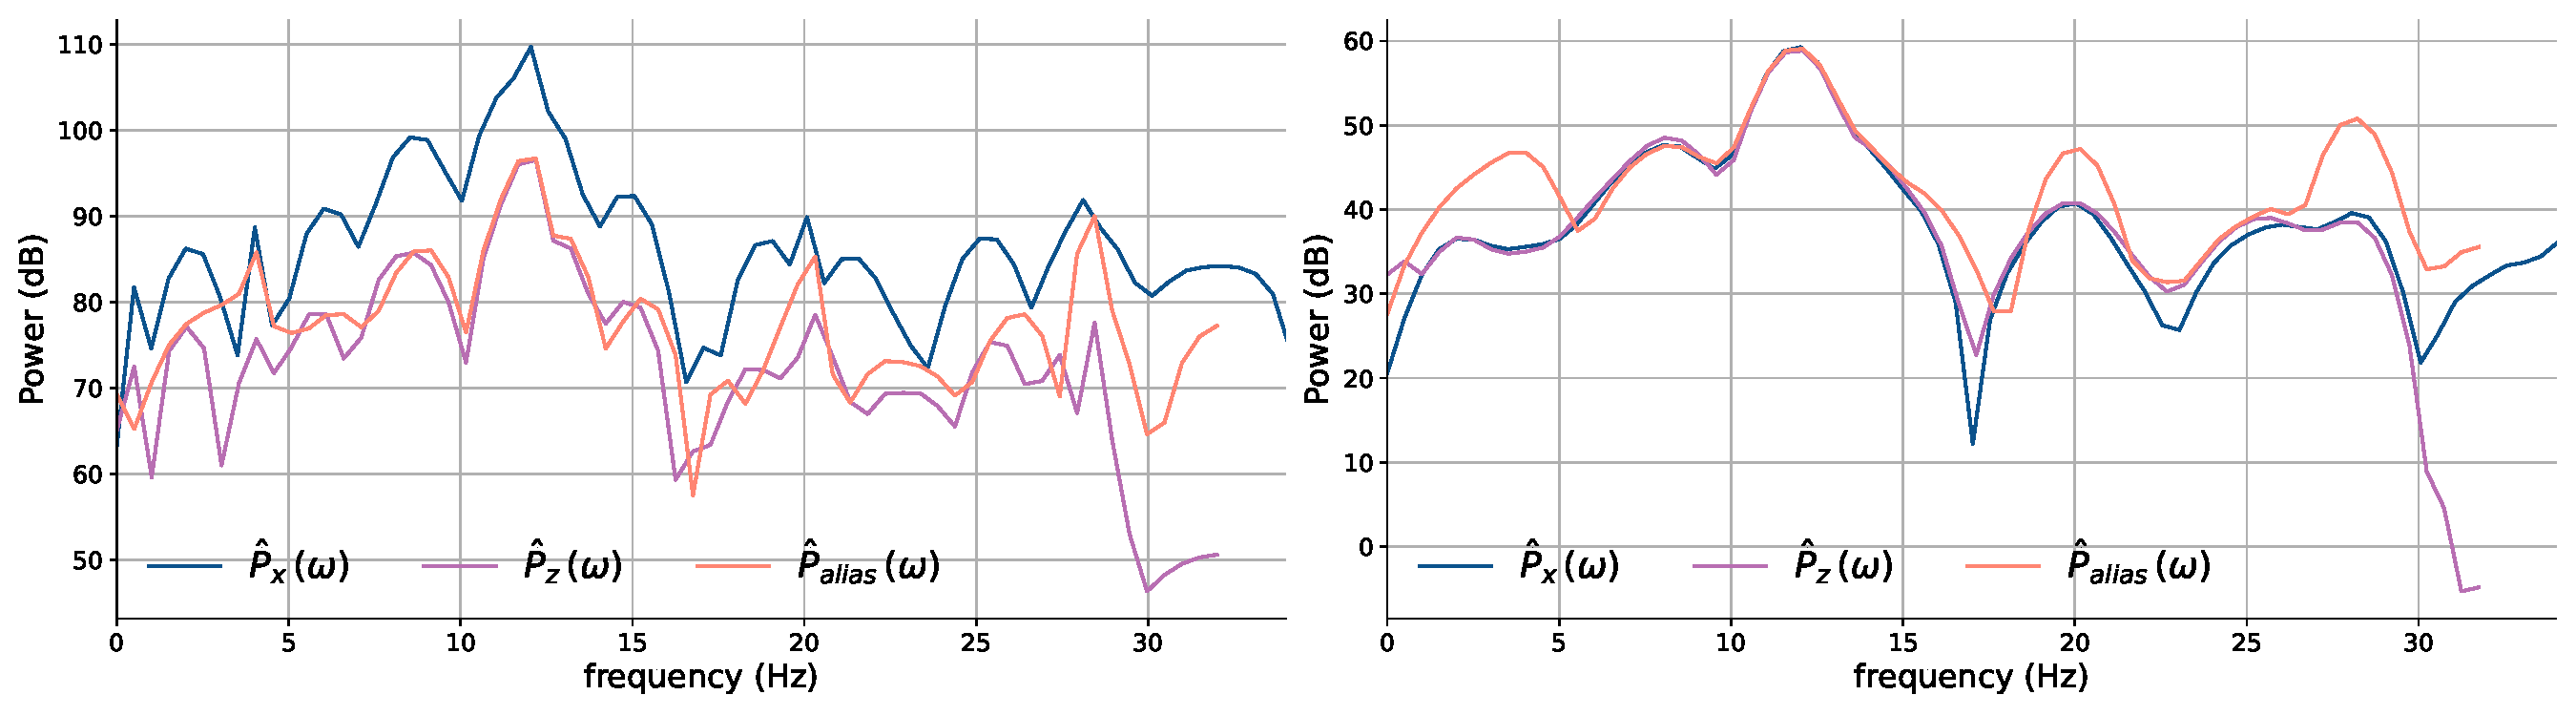
\includegraphics[width=\textwidth]{sq_wave_filtering_ds_spectra}
    \caption[PSD estimates of an input signal, filtered and downsampled version and a downsampled version without filtering.]{Standard periodogram (left) and Welch-averaged periodogram (right) representing PSD estimates $\hat{P}_x(\omega)$ and $\hat{P}_z(\omega)$ of input $x[n]$ and filtered, downsampled output $z[n]$ respectively. $\hat{P}_{\text{alias}}(\omega)$ shows the estimated spectrum of a downsampled version of $x[n]$ \textit{without} prior low-pass filtering}.
    \label{fig:sq-wave-ds-spectra-c6}
\end{figure}

\subsection{Hardware and data acquisition}

\begin{figure}[htp]
\subfloat[eyes open]{%
  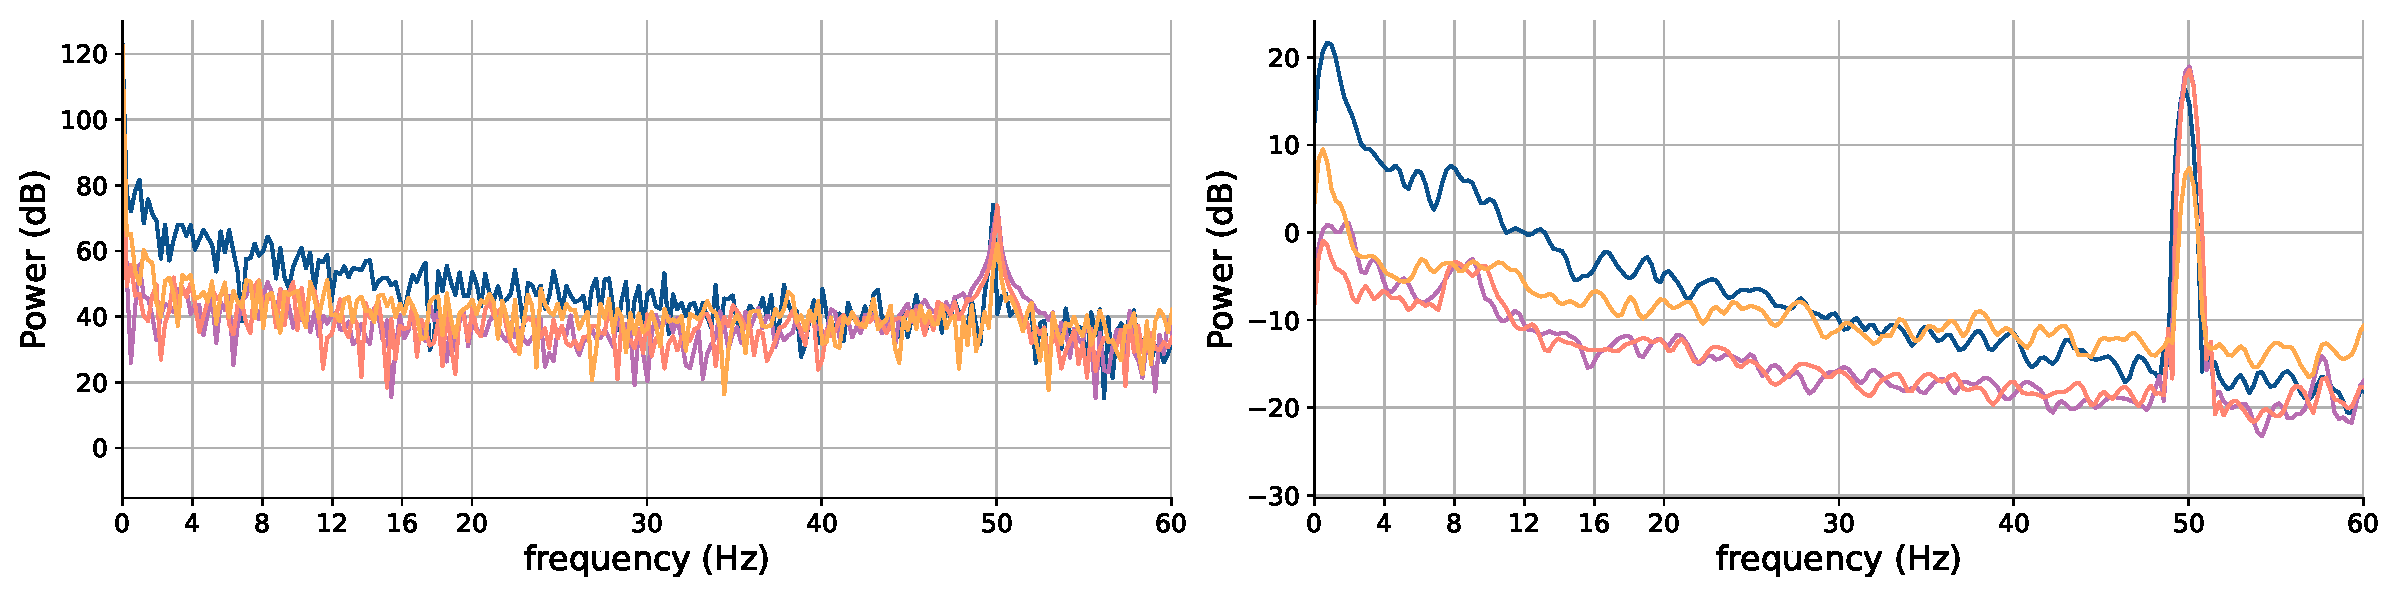
\includegraphics[clip,width=\columnwidth]{eyes_open_alpha_spectra_N1024.pdf}%
}

\subfloat[eyes closed]{%
  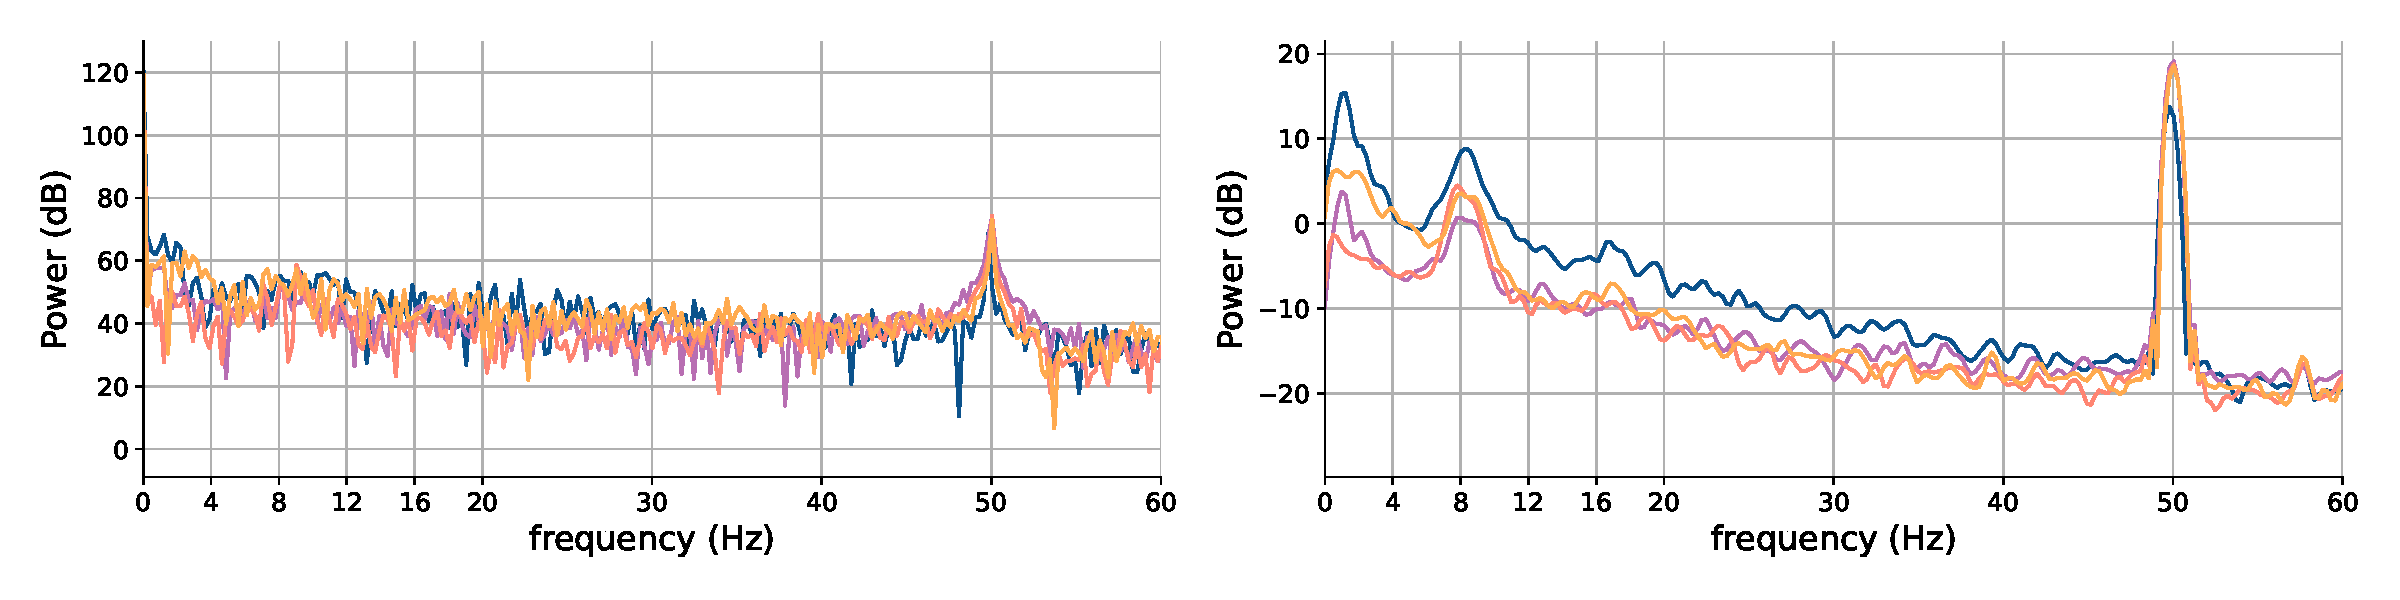
\includegraphics[clip,width=\columnwidth]{eyes_closed_alpha_spectra_N1024.pdf}%
}
\caption[\textbf{Alpha band test}: periodograms showing $N=1024$ point PSD estimates for EEG signals measured from a subject in two distinct states: with eyes open and eyes closed.]{\textbf{Alpha band test}: periodograms showing $N=1024$ point PSD estimates for EEG signals measured from a subject in two distinct states: with eyes open and eyes closed. Data was acquired using the early hardware prototype in Figure \ref{fig:frakenstein-hardware}. Attention should be given to signal power around $8-10$Hz (alpha band). In both (a) and (b), the left subplot shows a standard, non-windowed periodogram accompanied by a Welch-averaged periodogram to the right. Different coloured traces represent independent trials.}
\end{figure}


\section{Experimental Decoding Results}

%% Experiments with varying Nt: GCCA
\begin{figure}[htp]
\subfloat[$T = 0.75$s ($N_s=192, N_s'=48$)]{%
    \label{subfig:gcca-nt-ns48}
    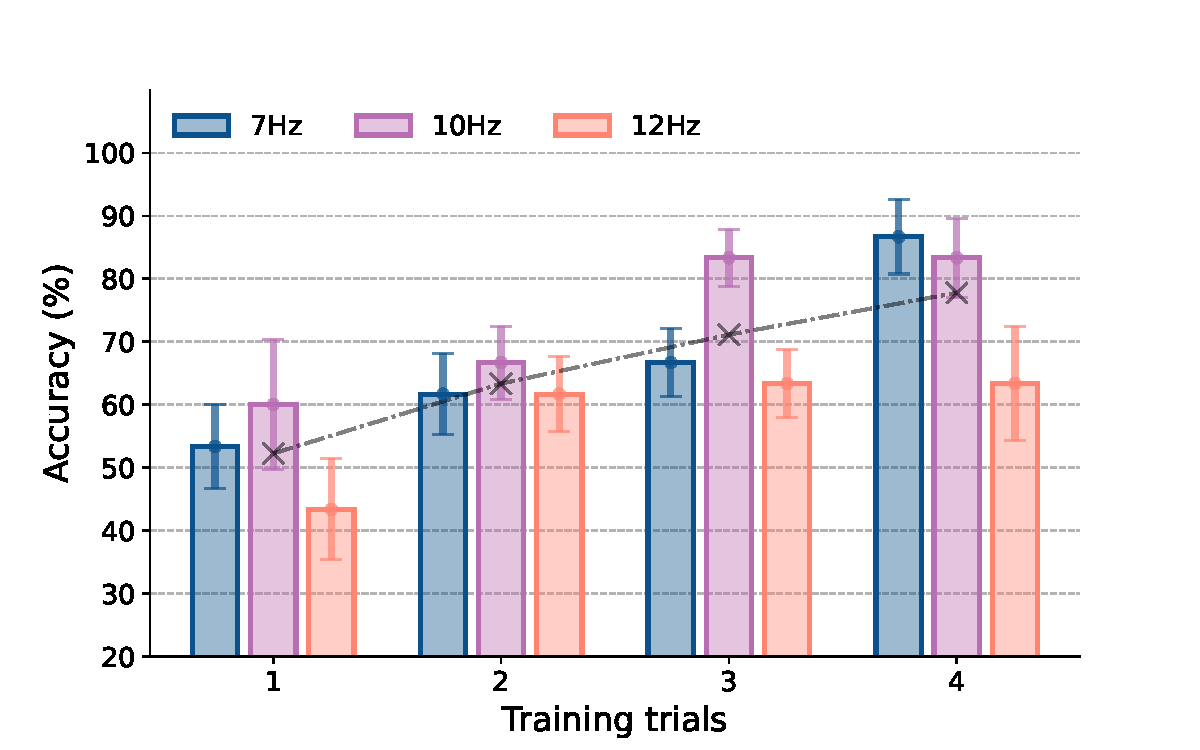
\includegraphics[clip,width=0.49\columnwidth]{report/C6 Results/assets/acc_Nt_gcca_Ns48.pdf}%
    \label{subfig:gcca-nt-ns64}
}
\hfill
\subfloat[$T = 1$s ($N_s=256, N_s'=64$)]{%
    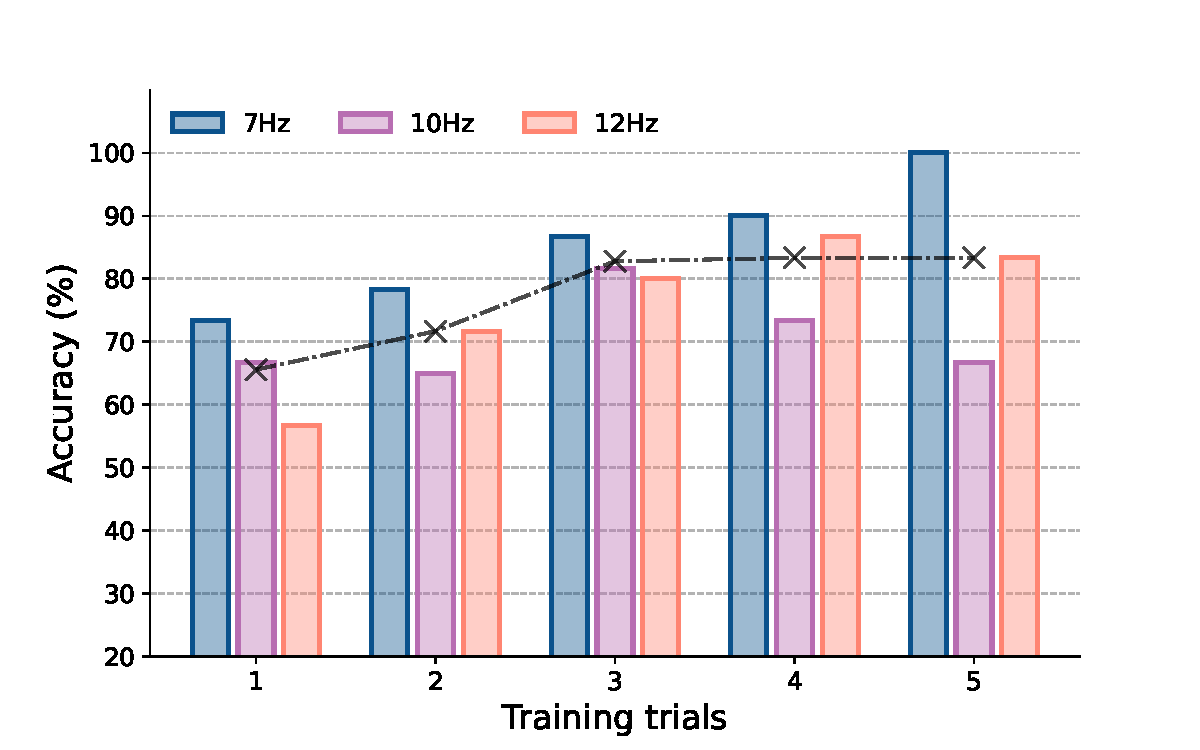
\includegraphics[clip,width=0.49\columnwidth]{report/C6 Results/assets/acc_Nt_gcca_Ns64.pdf}%
    \label{subfig:gcca-nt-ns64}
}
% ensure there is a space below here!

\subfloat[$T = 2$s ($N_s=512, N_s'=128$)]{%
    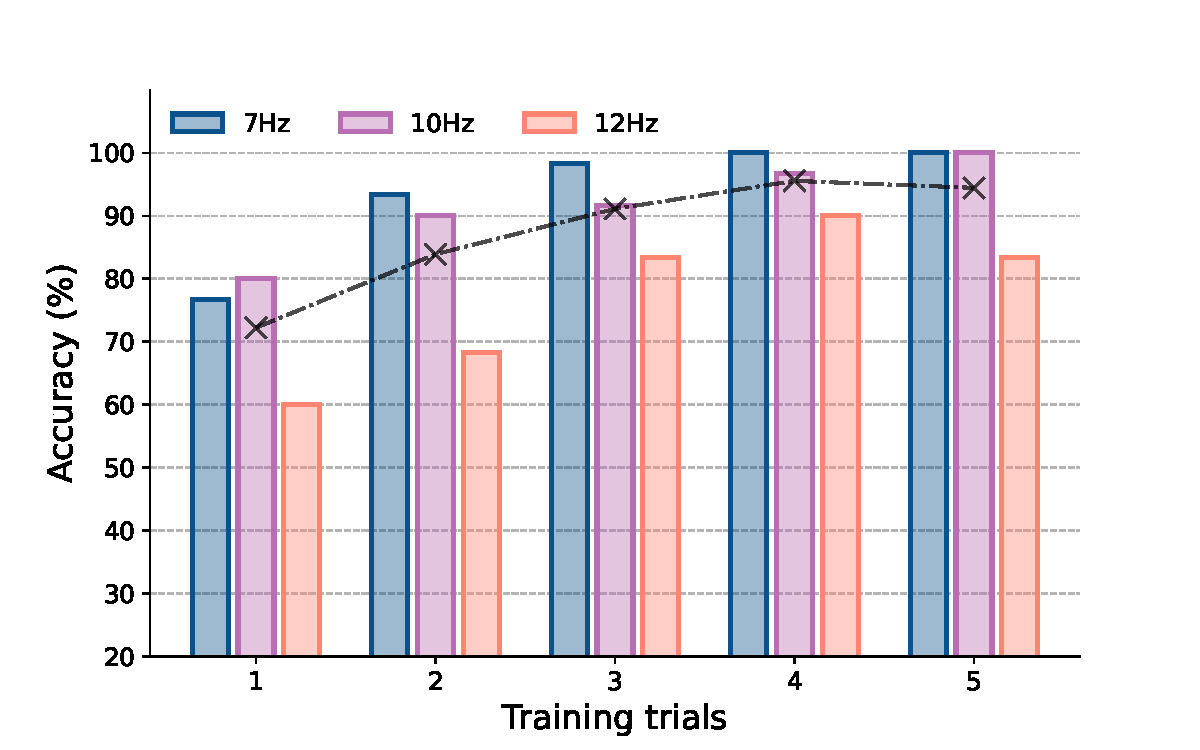
\includegraphics[clip,width=0.49\columnwidth]{report/C6 Results/assets/acc_Nt_gcca_Ns128.pdf}%
    \label{subfig:gcca-nt-ns128}
}
\hfill
\subfloat[$T = 4$s ($N_s=1024, N_s'=256$)]{%
    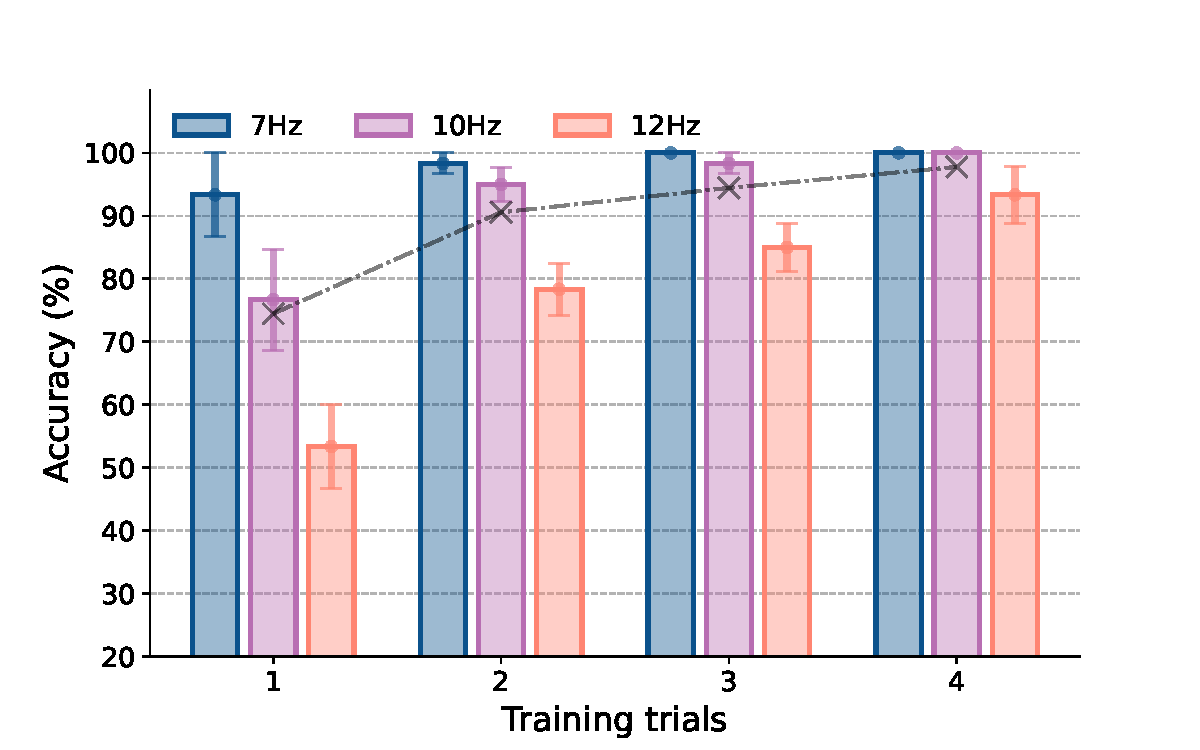
\includegraphics[clip,width=0.49\columnwidth]{report/C6 Results/assets/acc_Nt_gcca_Ns256.pdf}%
    \label{subfig:gcca-nt-ns256}
}

\caption[\textbf{GCCA decoding accuracy}: effect of varying the number of training (calibration) trials $N_t$ on validation accuracy for recording windows of varying length $T$.]{\textbf{GCCA decoding accuracy}: effect of varying the number of training (calibration) trials $N_t$ on validation accuracy for recording windows of varying length $T$. In each subfigure, all trials are of equal length $T$ seconds which equates to $N_s$ samples at $f_s=256$Hz and $N_s'$ samples at the downsampled rate of $f_s'=64$Hz. Crosses connected with dashed traces denote average decoding accuracy across stimulus frequencies for a given $N_t=n, \, n\in\{1, \dots, 5\}$.}
\label{fig:gcca-acc-nt}
\end{figure}


%% Experiments with varying Nt: MsetCCA
\begin{figure}[htp]
\subfloat[$T = 0.75$s ($N_s=192, N_s'=48$)]{%
    \label{subfig:gcca-nt-ns48}
    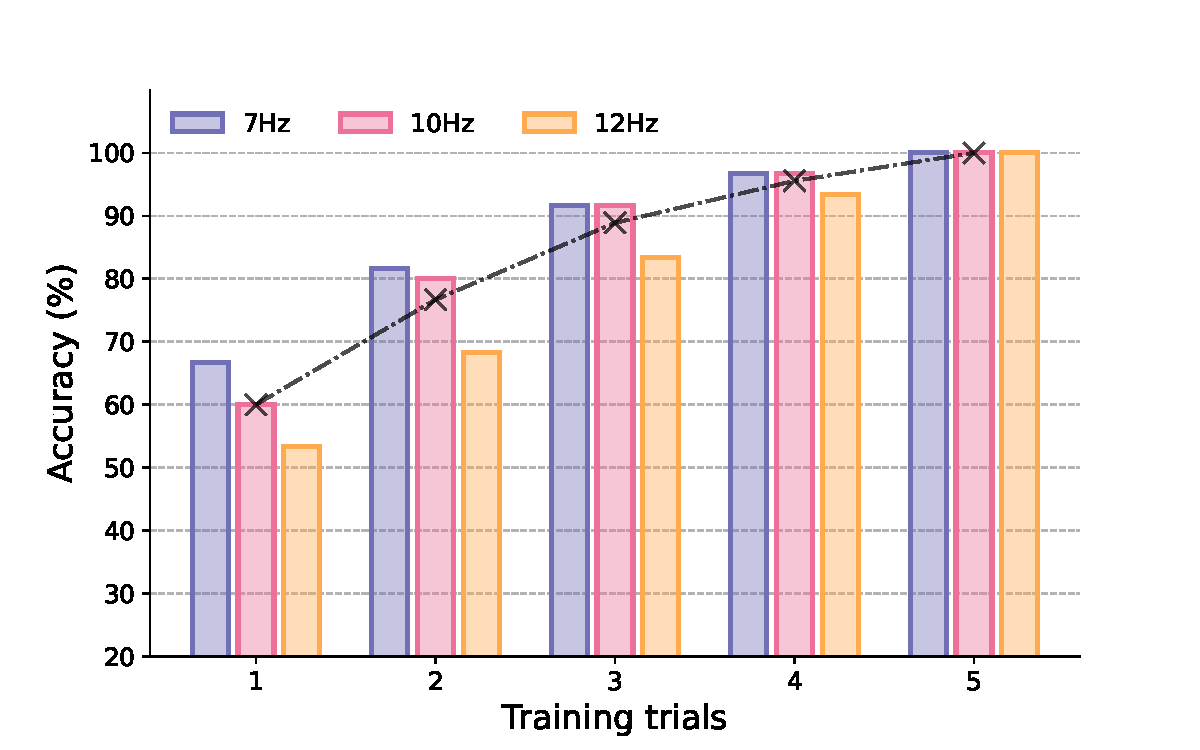
\includegraphics[clip,width=0.49\columnwidth]{report/C6 Results/assets/acc_Nt_mcca_Ns48.pdf}%
}
\hfill
\subfloat[$T = 1$s ($N_s=256, N_s'=64$)]{%
    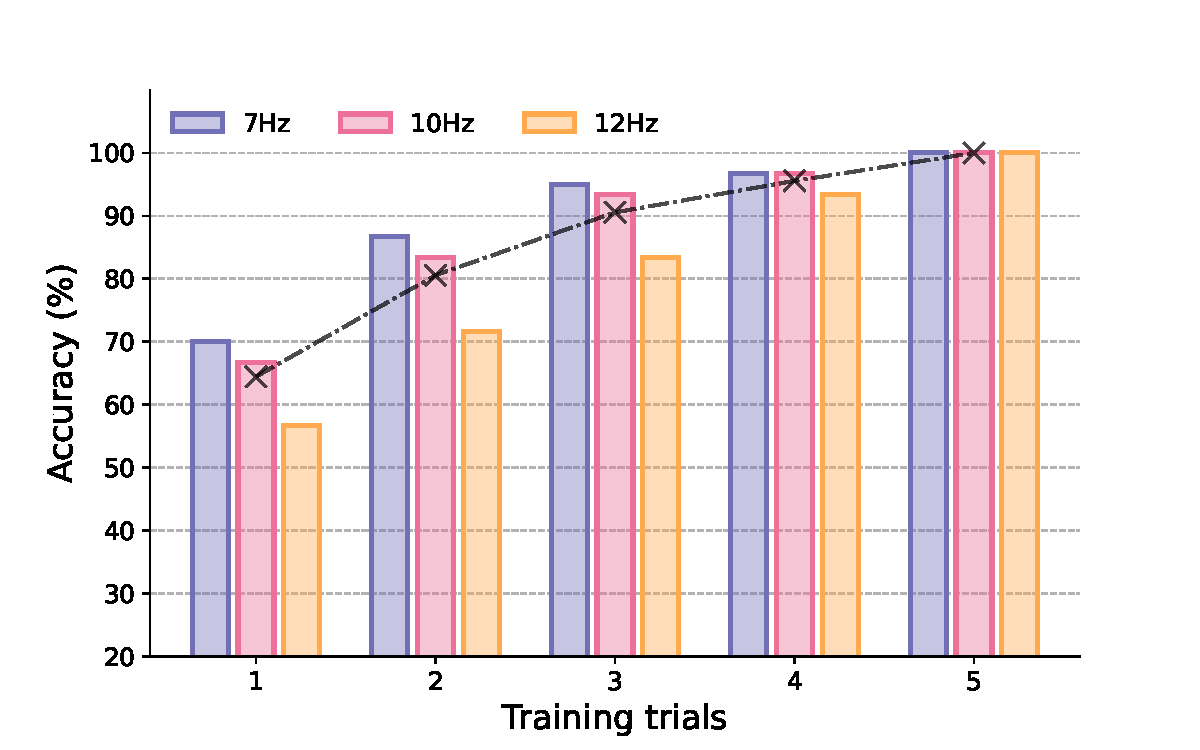
\includegraphics[clip,width=0.49\columnwidth]{report/C6 Results/assets/acc_Nt_mcca_Ns64.pdf}%
    \label{subfig:mset-nt-ns64}
}
% ensure there is a space below here!

\subfloat[$T = 2$s ($N_s=512, N_s'=128$)]{%
    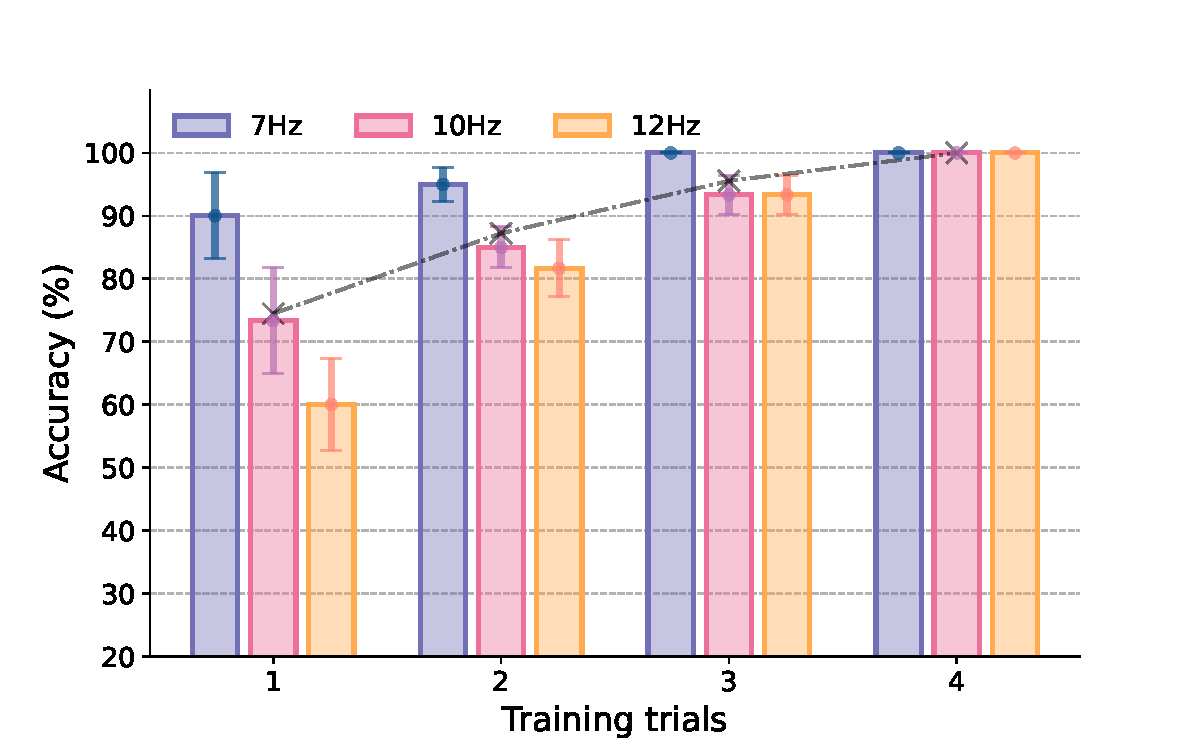
\includegraphics[clip,width=0.49\columnwidth]{report/C6 Results/assets/acc_Nt_mcca_Ns128.pdf}%
    \label{subfig:mset-nt-ns128}
}
\hfill
\subfloat[$T = 4$s ($N_s=1024, N_s'=256$)]{%
    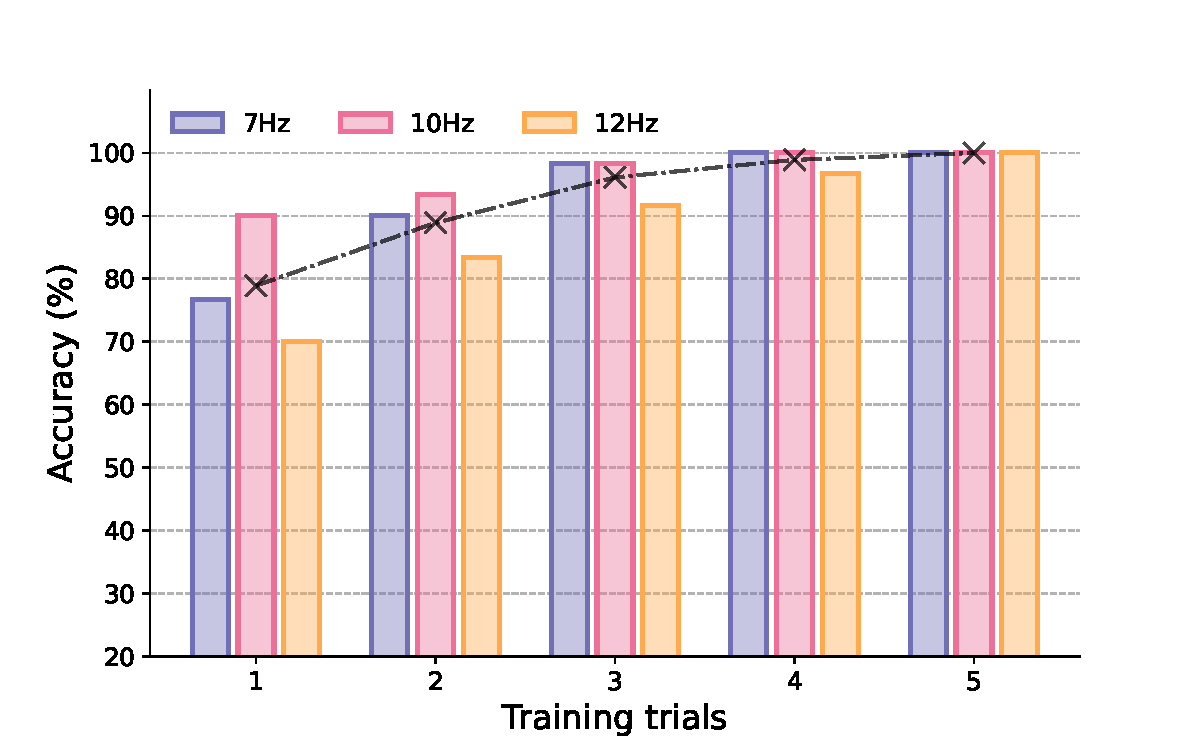
\includegraphics[clip,width=0.49\columnwidth]{report/C6 Results/assets/acc_Nt_mcca_Ns256.pdf}%
    \label{subfig:mset-nt-ns256}
}

\caption[\textbf{MsetCCA decoding accuracy}: effect of varying the number of training (calibration) trials $N_t$ on validation accuracy for recording windows of varying length $T$.]{\textbf{MsetCCA decoding accuracy}: effect of varying the number of training (calibration) trials $N_t$ on validation accuracy for recording windows of varying length $T$. In each subfigure, all trials are of equal length $T$ seconds which equates to $N_s$ samples at $f_s=256$Hz and $N_s'$ samples at the downsampled rate of $f_s'=64$Hz. Crosses connected with dashed traces denote average decoding accuracy across stimulus frequencies for a given $N_t=n, \, n\in\{1, \dots, 5\}$.}
\label{fig:mset-acc-nt}
\end{figure}

%% [SAMPLING LENGTH] Experiments with varying Ns: GCCA
\begin{figure}[htp]
\subfloat[$N_t=1$]{%
    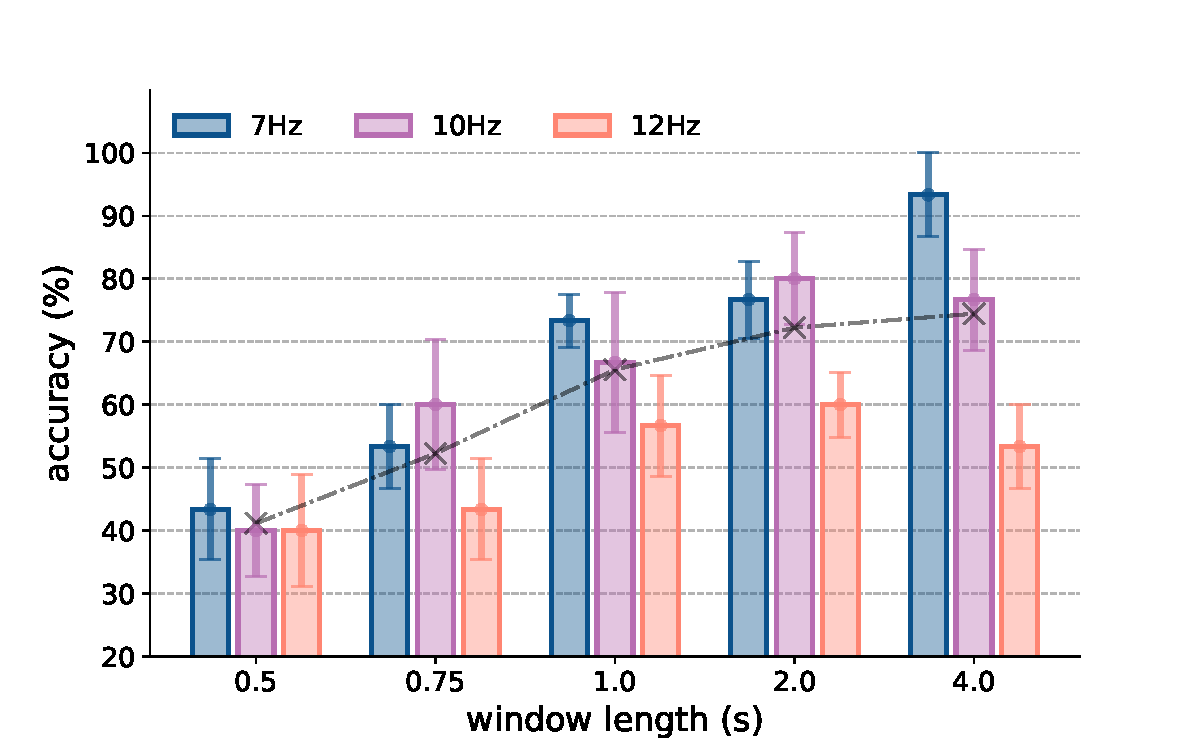
\includegraphics[clip,width=0.49\columnwidth]{report/C6 Results/assets/acc_Ns_gcca_Nt1.pdf}%
    \label{subfig:gcca-ns-nt1}
}
\hfill
\subfloat[$N_t=2$]{%
    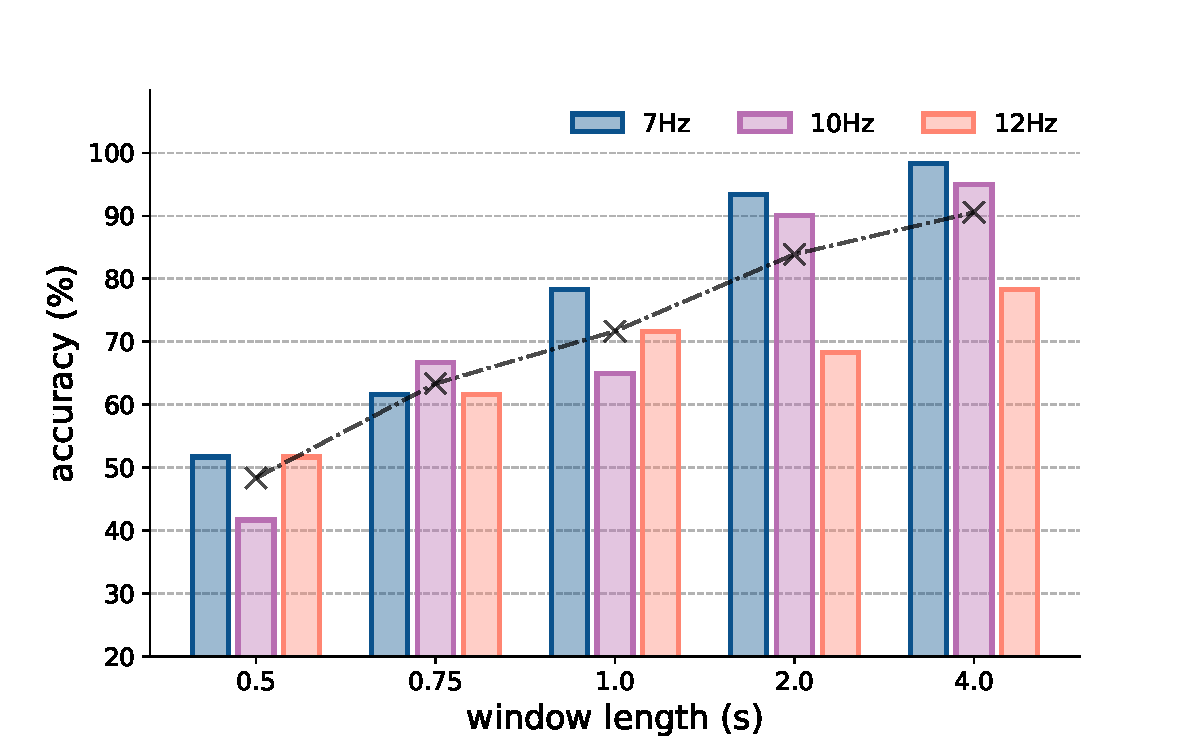
\includegraphics[clip,width=0.49\columnwidth]{report/C6 Results/assets/acc_Ns_gcca_Nt2.pdf}%
    \label{subfig:gcca-ns-nt2}
}
% ensure there is a space below here!

\subfloat[$N_t=3$)]{%
    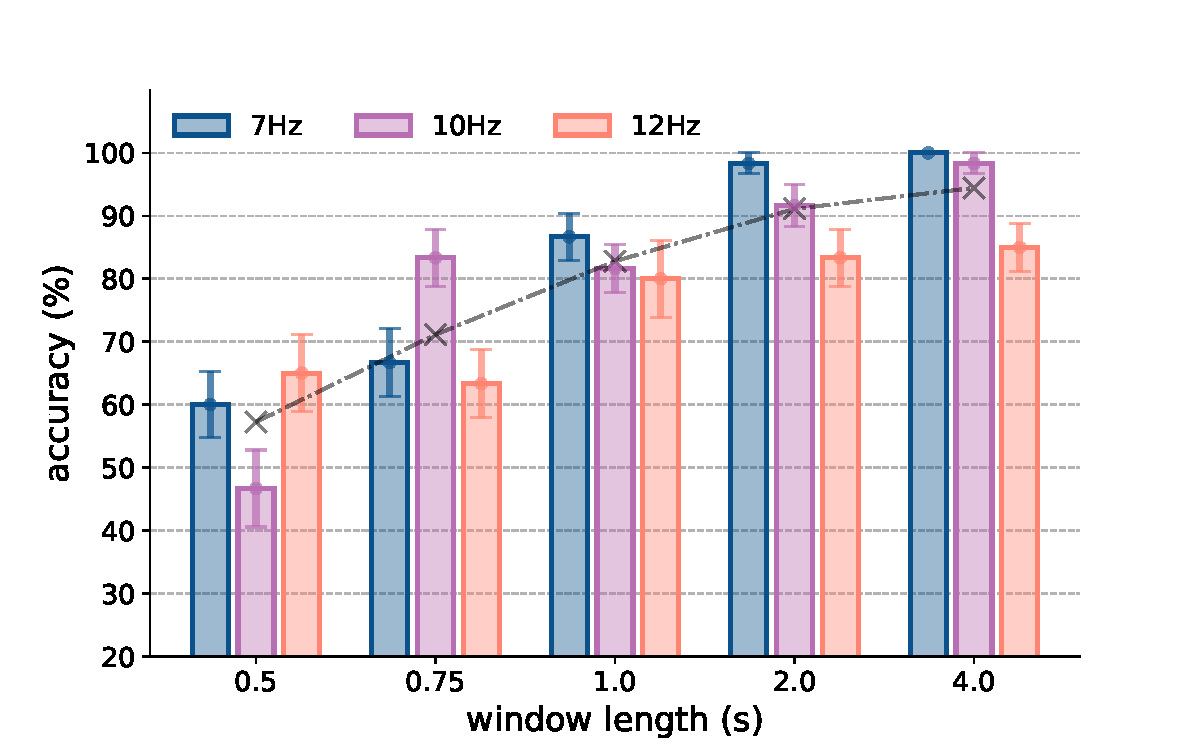
\includegraphics[clip,width=0.49\columnwidth]{report/C6 Results/assets/acc_Ns_gcca_Nt3.pdf}%
    \label{subfig:gcca-ns-nt3}
}
\hfill
\subfloat[$N_t=4$]{%
    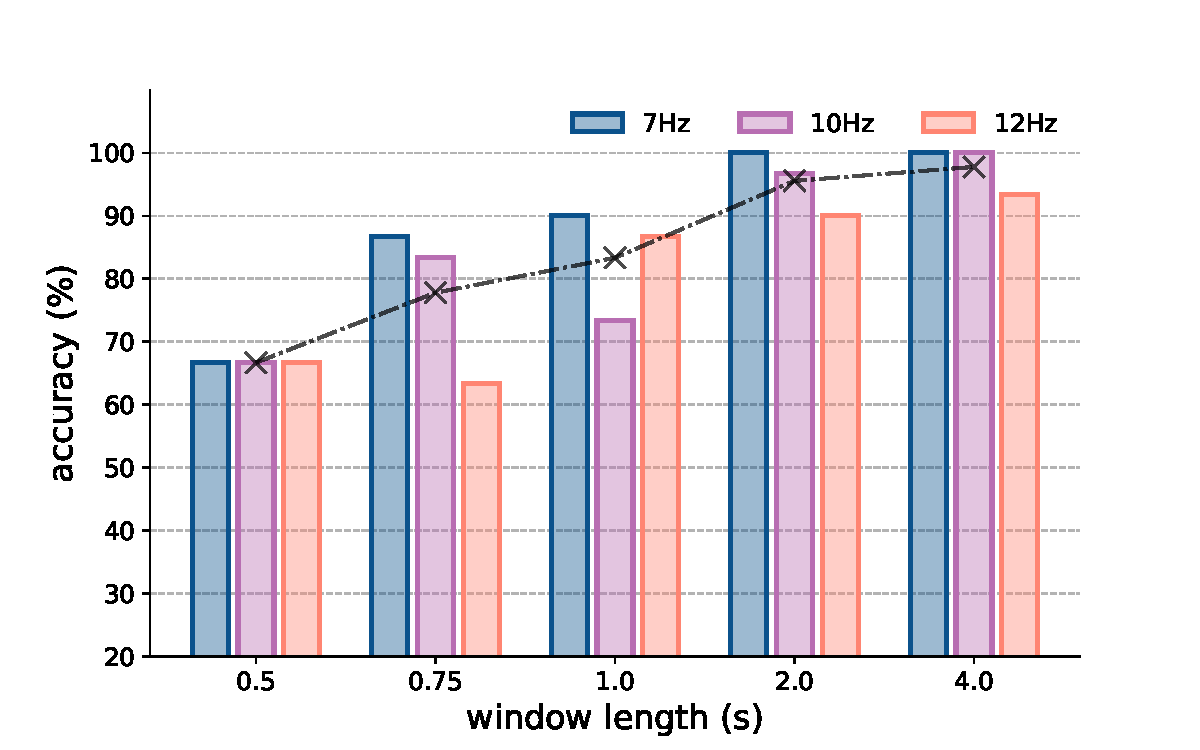
\includegraphics[clip,width=0.49\columnwidth]{report/C6 Results/assets/acc_Ns_gcca_Nt4.pdf}%
    \label{subfig:gcca-ns-nt4}
}

\caption[\textbf{GCCA decoding accuracy}: effect of varying recording window length $T$ on validation accuracy for different numbers of calibration trails $N_t$]{\textbf{GCCA decoding accuracy}: effect of varying recording window length $T$ on validation accuracy for different numbers of calibration trails $N_t$. In each subfigure, all results were computed using $N_t=n, \, n\in\{1, \dots, 4\}$ calibration trials. Crosses connected with dashed traces denote average decoding accuracy across stimulus frequencies for a given a given window length $T$.}
\label{fig:gcca-acc-ns}
\end{figure}

%% [SAMPLING LENGTH] Experiments with varying Ns: MsetCCA
\begin{figure}[htp]
\subfloat[$N_t=1$]{%
    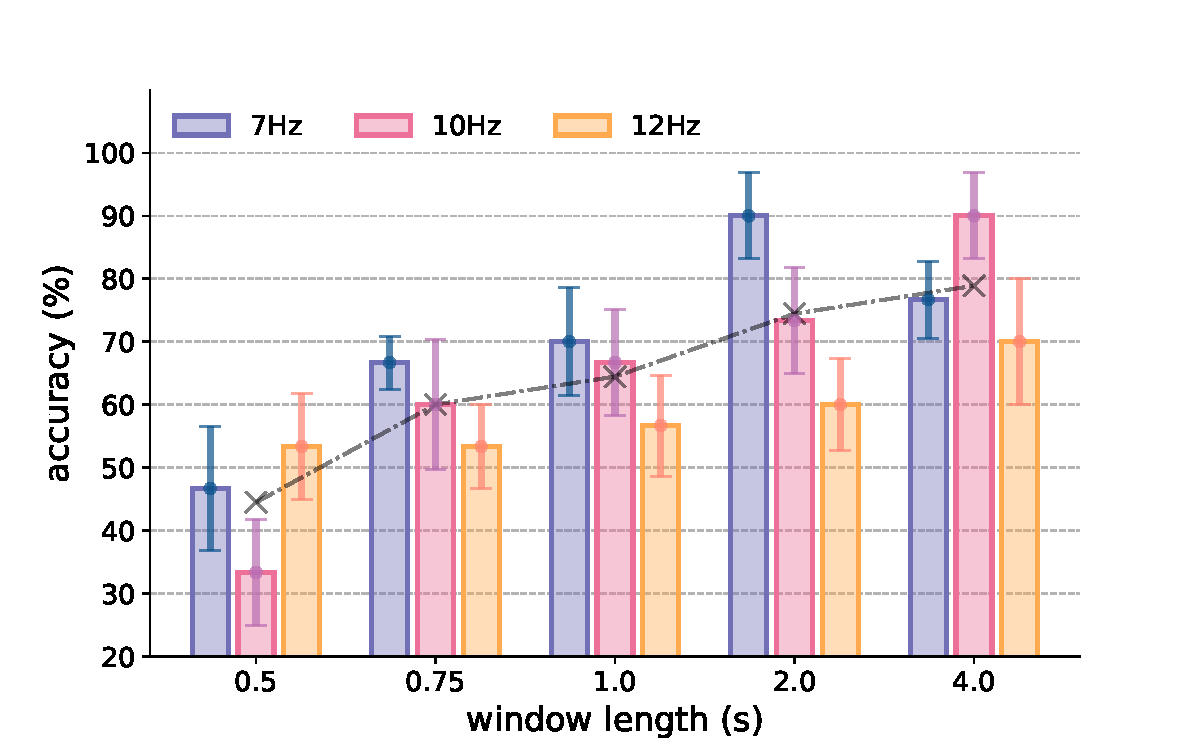
\includegraphics[clip,width=0.49\columnwidth]{report/C6 Results/assets/acc_Ns_mcca_Nt1.pdf}%
    \label{subfig:mcca-ns-nt1}
}
\hfill
\subfloat[$N_t=2$]{%
    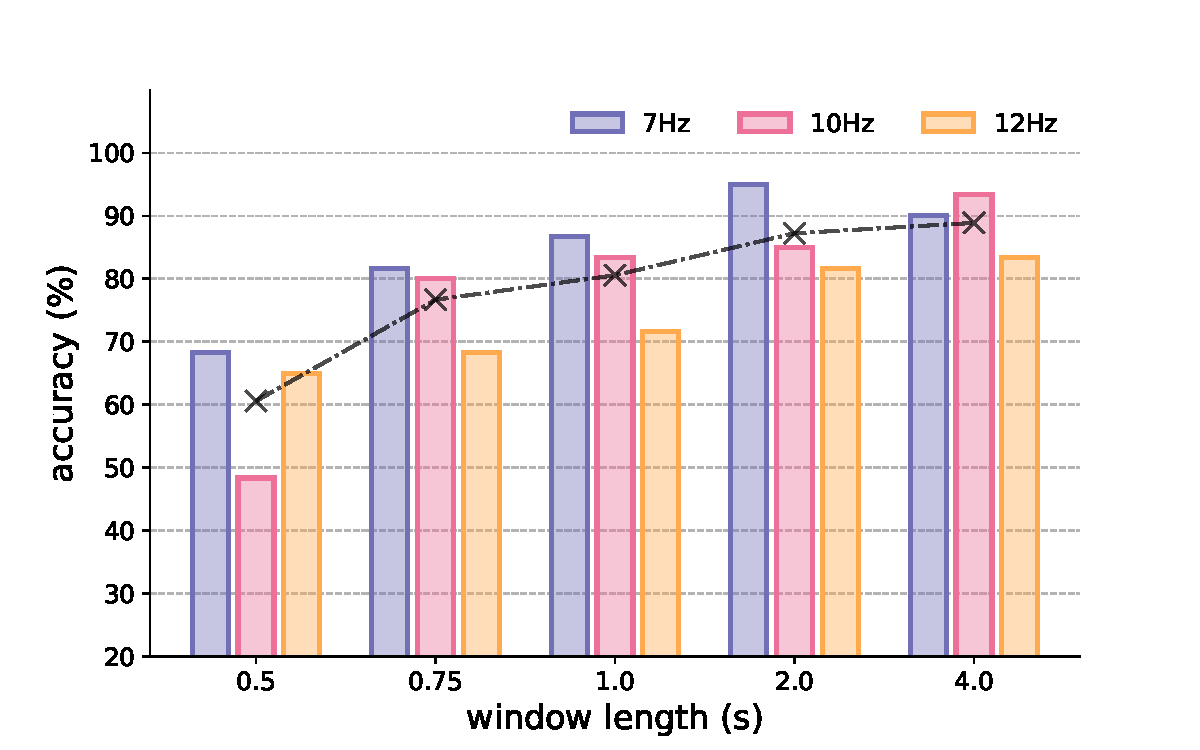
\includegraphics[clip,width=0.49\columnwidth]{report/C6 Results/assets/acc_Ns_mcca_Nt2.pdf}%
    \label{subfig:mcca-ns-nt2}
}
% ensure there is a space below here!

\subfloat[$N_t=3$)]{%
    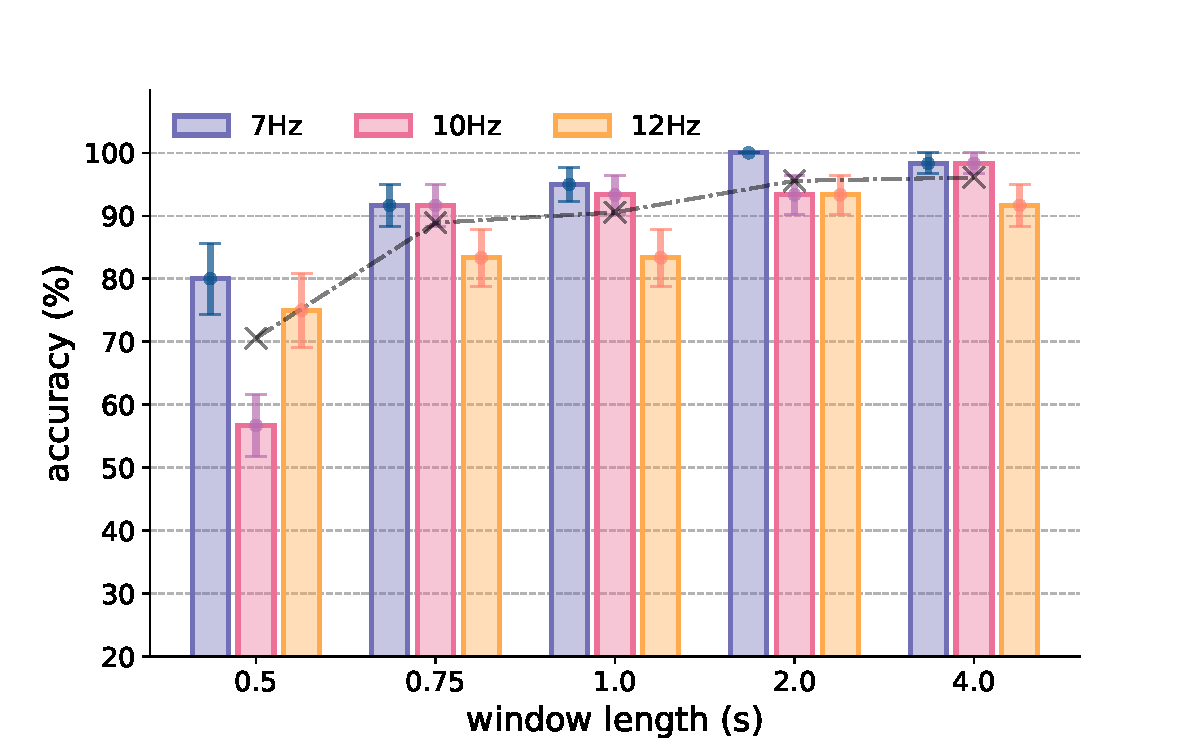
\includegraphics[clip,width=0.49\columnwidth]{report/C6 Results/assets/acc_Ns_mcca_Nt3.pdf}%
    \label{subfig:mcca-ns-nt3}
}
\hfill
\subfloat[$N_t=4$]{%
    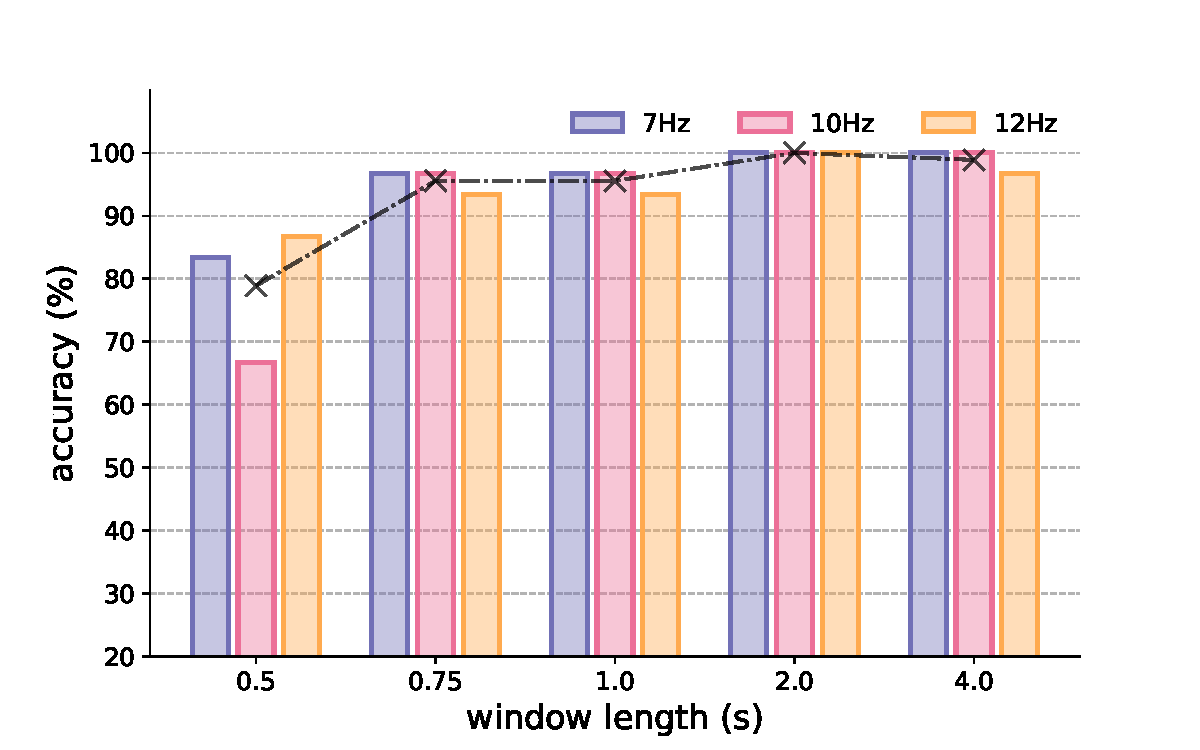
\includegraphics[clip,width=0.49\columnwidth]{report/C6 Results/assets/acc_Ns_mcca_Nt4.pdf}%
    \label{subfig:mcca-ns-nt4}
}

\caption[\textbf{MsetCCA decoding accuracy}: effect of varying recording window length $T$ on validation accuracy for different numbers of calibration trails $N_t$]{\textbf{MsetCCA decoding accuracy}: effect of varying recording window length $T$ on validation accuracy for different numbers of calibration trails $N_t$. In each subfigure, all results were computed using $N_t=n, \, n\in\{1, \dots, 4\}$ calibration trials. Crosses connected with dashed traces denote average decoding accuracy across stimulus frequencies for a given a given window length $T$.}
\label{fig:mcca-acc-ns}
\end{figure}

% \begin{figure}
%      \centering
%      \begin{subfigure}[b]{0.3\textwidth}
%          \centering
%          \includegraphics[width=\textwidth]{acc}
%          \caption{$y=x$}
%          \label{fig:y equals x}
%      \end{subfigure}
%      \hfill
%      \begin{subfigure}[b]{0.3\textwidth}
%          \centering
%          \includegraphics[width=\textwidth]{graph2}
%          \caption{$y=3sinx$}
%          \label{fig:three sin x}
%      \end{subfigure}
%      \hfill
%      \begin{subfigure}[b]{0.3\textwidth}
%          \centering
%          \includegraphics[width=\textwidth]{graph3}
%          \caption{$y=5/x$}
%          \label{fig:five over x}
%      \end{subfigure}
%         \caption{Three simple graphs}
%         \label{fig:three graphs}
% \end{figure}

% \section{Experiments using Benchmark Data}
